\documentclass[11pt,colorlinks]{charlie}
\usepackage{booktabs,array}
\newcolumntype{L}[1]{>{\raggedright\arraybackslash}p{#1}}
\setlength{\emergencystretch}{3em}
\usepackage[capitalize,nameinlink]{cleveref}
\usepackage{aliascnt}
\makeatletter
\def\ch@redefthm#1#2#3{\expandafter\let\csname #1\endcsname\relax
  \expandafter\let\csname end#1\endcsname\relax
  \newaliascnt{#1}{theorem}\newtheorem{#1}[#1]{#2}\aliascntresetthe{#1}%
  \crefname{#1}{#2}{#3}\Crefname{#1}{#2}{#3}}
\crefname{theorem}{Theorem}{Theorems}\Crefname{theorem}{Theorem}{Theorems}
\theoremstyle{chplain}
\ch@redefthm{lemma}{Lemma}{Lemmas}
\ch@redefthm{proposition}{Proposition}{Propositions}
\ch@redefthm{corollary}{Corollary}{Corollaries}
\ch@redefthm{conjecture}{Conjecture}{Conjectures}
\theoremstyle{chdefinition}
\ch@redefthm{definition}{Definition}{Definitions}
\ch@redefthm{example}{Example}{Examples}
\ch@redefthm{hypothesis}{Hypothesis}{Hypotheses}
\makeatother

\newcommand{\R}{\mathbb{R}}
\newcommand{\C}{\mathbb{C}}
\newcommand{\Z}{\mathbb{Z}}
\newcommand{\Q}{\mathbb{Q}}
\newcommand{\N}{\mathbb{N}}
\newcommand{\E}{\mathbb{E}}
\newcommand{\one}{\mathbf{1}}
\newcommand{\dd}{\,\mathrm{d}}

\newif\ifdraftmarkers \draftmarkersfalse
\newcounter{gapcount}
\newcommand{\gap}[1]{\ifdraftmarkers\stepcounter{gapcount}%
  \par\smallskip\noindent\fcolorbox{red!60!black}{red!5}{\parbox{\dimexpr\linewidth-2\fboxsep-2\fboxrule}{%
  \textcolor{red!60!black}{\textbf{Gap \thegapcount.}} #1}}\par\smallskip\fi}
\newcommand{\unchecked}[1]{\ifdraftmarkers%
  \par\smallskip\noindent\fcolorbox{orange!80!black}{orange!6}{\parbox{\dimexpr\linewidth-2\fboxsep-2\fboxrule}{%
  \textcolor{orange!80!black}{\textbf{Unchecked.}} #1}}\par\smallskip\fi}
\newcommand{\source}[1]{\ifdraftmarkers{\textcolor{gray}{\footnotesize[source: \texttt{#1}]}}\fi}
\newcommand{\todo}[1]{\ifdraftmarkers{\textcolor{blue!70!black}{\footnotesize[\textbf{todo:} #1]}}\fi}

\newcommand{\coderepo}{\url{https://github.com/charlieoneill11/maths-releases}}
\newcommand{\aiusestatement}{The mathematical arguments and computer programs in this paper were developed by Astra (GPT-6.2 Astra, OpenAI). Fable (Fable~5.2, Anthropic) worked throughout as a second model: it proposed alternative approaches, reviewed arguments and raised objections. The manuscript was prepared from the project's research records with Claude (Anthropic). All computations were re-run before release, and the programs and certificates are available at \coderepo.}
\newcommand{\responsibilitystatement}{Charles O'Neill has checked the arguments and takes full responsibility for the correctness of the results.}
\newcommand{\mscandkeywords}[2]{\par\medskip\noindent{\small\textit{2020 Mathematics Subject Classification.} #1\par\noindent\textit{Keywords.} #2\par}}

\usepackage{amssymb}
\usepackage{graphicx}

\newcommand{\F}{\mathbb{F}}
\newcommand{\T}{\mathsf T}
\newcommand{\dev}[1]{[#1]}
\renewcommand{\aiusestatement}{The construction and the search and verification programs in this paper were developed and run by Astra (GPT-6.2 Astra, OpenAI) from Charles O'Neill's instructions, starting from Kishan Kumar's public search programs. The manuscript was prepared from the project's research records with Claude (Anthropic). All computations were re-run before release, and the programs, the certificate and the matrix are available at \coderepo.}

\title{A Hadamard matrix of order 4792}
\author{Charles O'Neill, Max Kirkby and Astra}
\date{25 November 2026}

\begin{document}
\maketitle

\begin{abstract}
We construct a Hadamard matrix of order $4792=8\cdot599$, an order for which no Hadamard matrix was previously known. The order is twice $2396$, the smallest order for which no Hadamard matrix is known, and it was one of the last two open orders of the form $8p$ below $10\,000$. The matrix is a Goethals--Seidel array with a border, built from four $\pm1$ functions on the abelian group $\Z_7\times\Z_{19}\times\F_9$ of order $1197$ whose periodic autocorrelations sum to $-4$ at every nonzero shift. The four functions are invariant under a group of multipliers of order $36$, so they are given by twelve $17$-bit masks. We verify the autocorrelation identity by counting differences, and we check that $HH^{\T}=4792I$ with three independent programs. The functions were found by a computer search in a family of symmetric structures proposed by Kumar, who used the same construction to give a Hadamard matrix of order $5912=8\cdot739$.
\end{abstract}
\mscandkeywords{05B20; 05B10, 15B34}{Hadamard matrix, Goethals--Seidel array, supplementary difference sets, periodic autocorrelation, computer search}

\section*{AI use and author contributions}
\aiusestatement

Charles O'Neill chose the problem and directed the search. \responsibilitystatement

\section{Introduction}
A \emph{Hadamard matrix} of order $n$ is an $n\times n$ matrix $H$ with entries $\pm1$ and $HH^{\T}=nI$. Such a matrix can exist only for $n=1$, $n=2$ and $n\equiv0\pmod4$ \cite{Hadamard}, and the Hadamard conjecture, first stated by Paley \cite{Paley}, asserts that it exists for every such $n$. Sylvester's doubling \cite{Sylvester} turns a Hadamard matrix of order $n$ into one of order $2n$, Paley's constructions \cite{Paley} cover orders $q+1$ and $2(q+1)$ for suitable prime powers $q$, and a long list of further constructions, many of them computer searches over arrays of commuting blocks, covers most other small orders; see \cite{SY,EKLO}. In 2005 Kharaghani and Tayfeh-Rezaie found a Hadamard matrix of order $428$ \cite{KTR}, and $668$ remained the smallest open order for about twenty years. In 2026 many of the smallest open orders were settled; the survey of Egan, Kotsireas, London and \'O Cath\'ain \cite{EKLO} and Kumar's tally \cite{Kumar} record them.

As of 25 November 2026, the smallest order for which no Hadamard matrix is known is $2396=4\cdot599$ \cite{Explorer,Kumar}. Twice that order was open as well: the Hadamard Matrix Explorer lists $4792$ as unknown \cite{Explorer}, and Kumar's search records \cite{Kumar} list $4792=8\cdot599$ and $5752=8\cdot719$ as the two remaining open orders of the form $8p$ below $10\,000$, after his construction of order $5912=8\cdot739$. We settle this order.

\begin{theorem}\label{thm:main}
There is a Hadamard matrix of order $4792$.
\end{theorem}

A Hadamard matrix of order $2396$ would give one of order $4792$ by doubling. Our matrix does not arise in this way, and order $2396$ remains open. \Cref{fig:matrix} shows the matrix.

\begin{figure}[ht]
\centering
\begin{minipage}[b]{0.62\linewidth}\centering
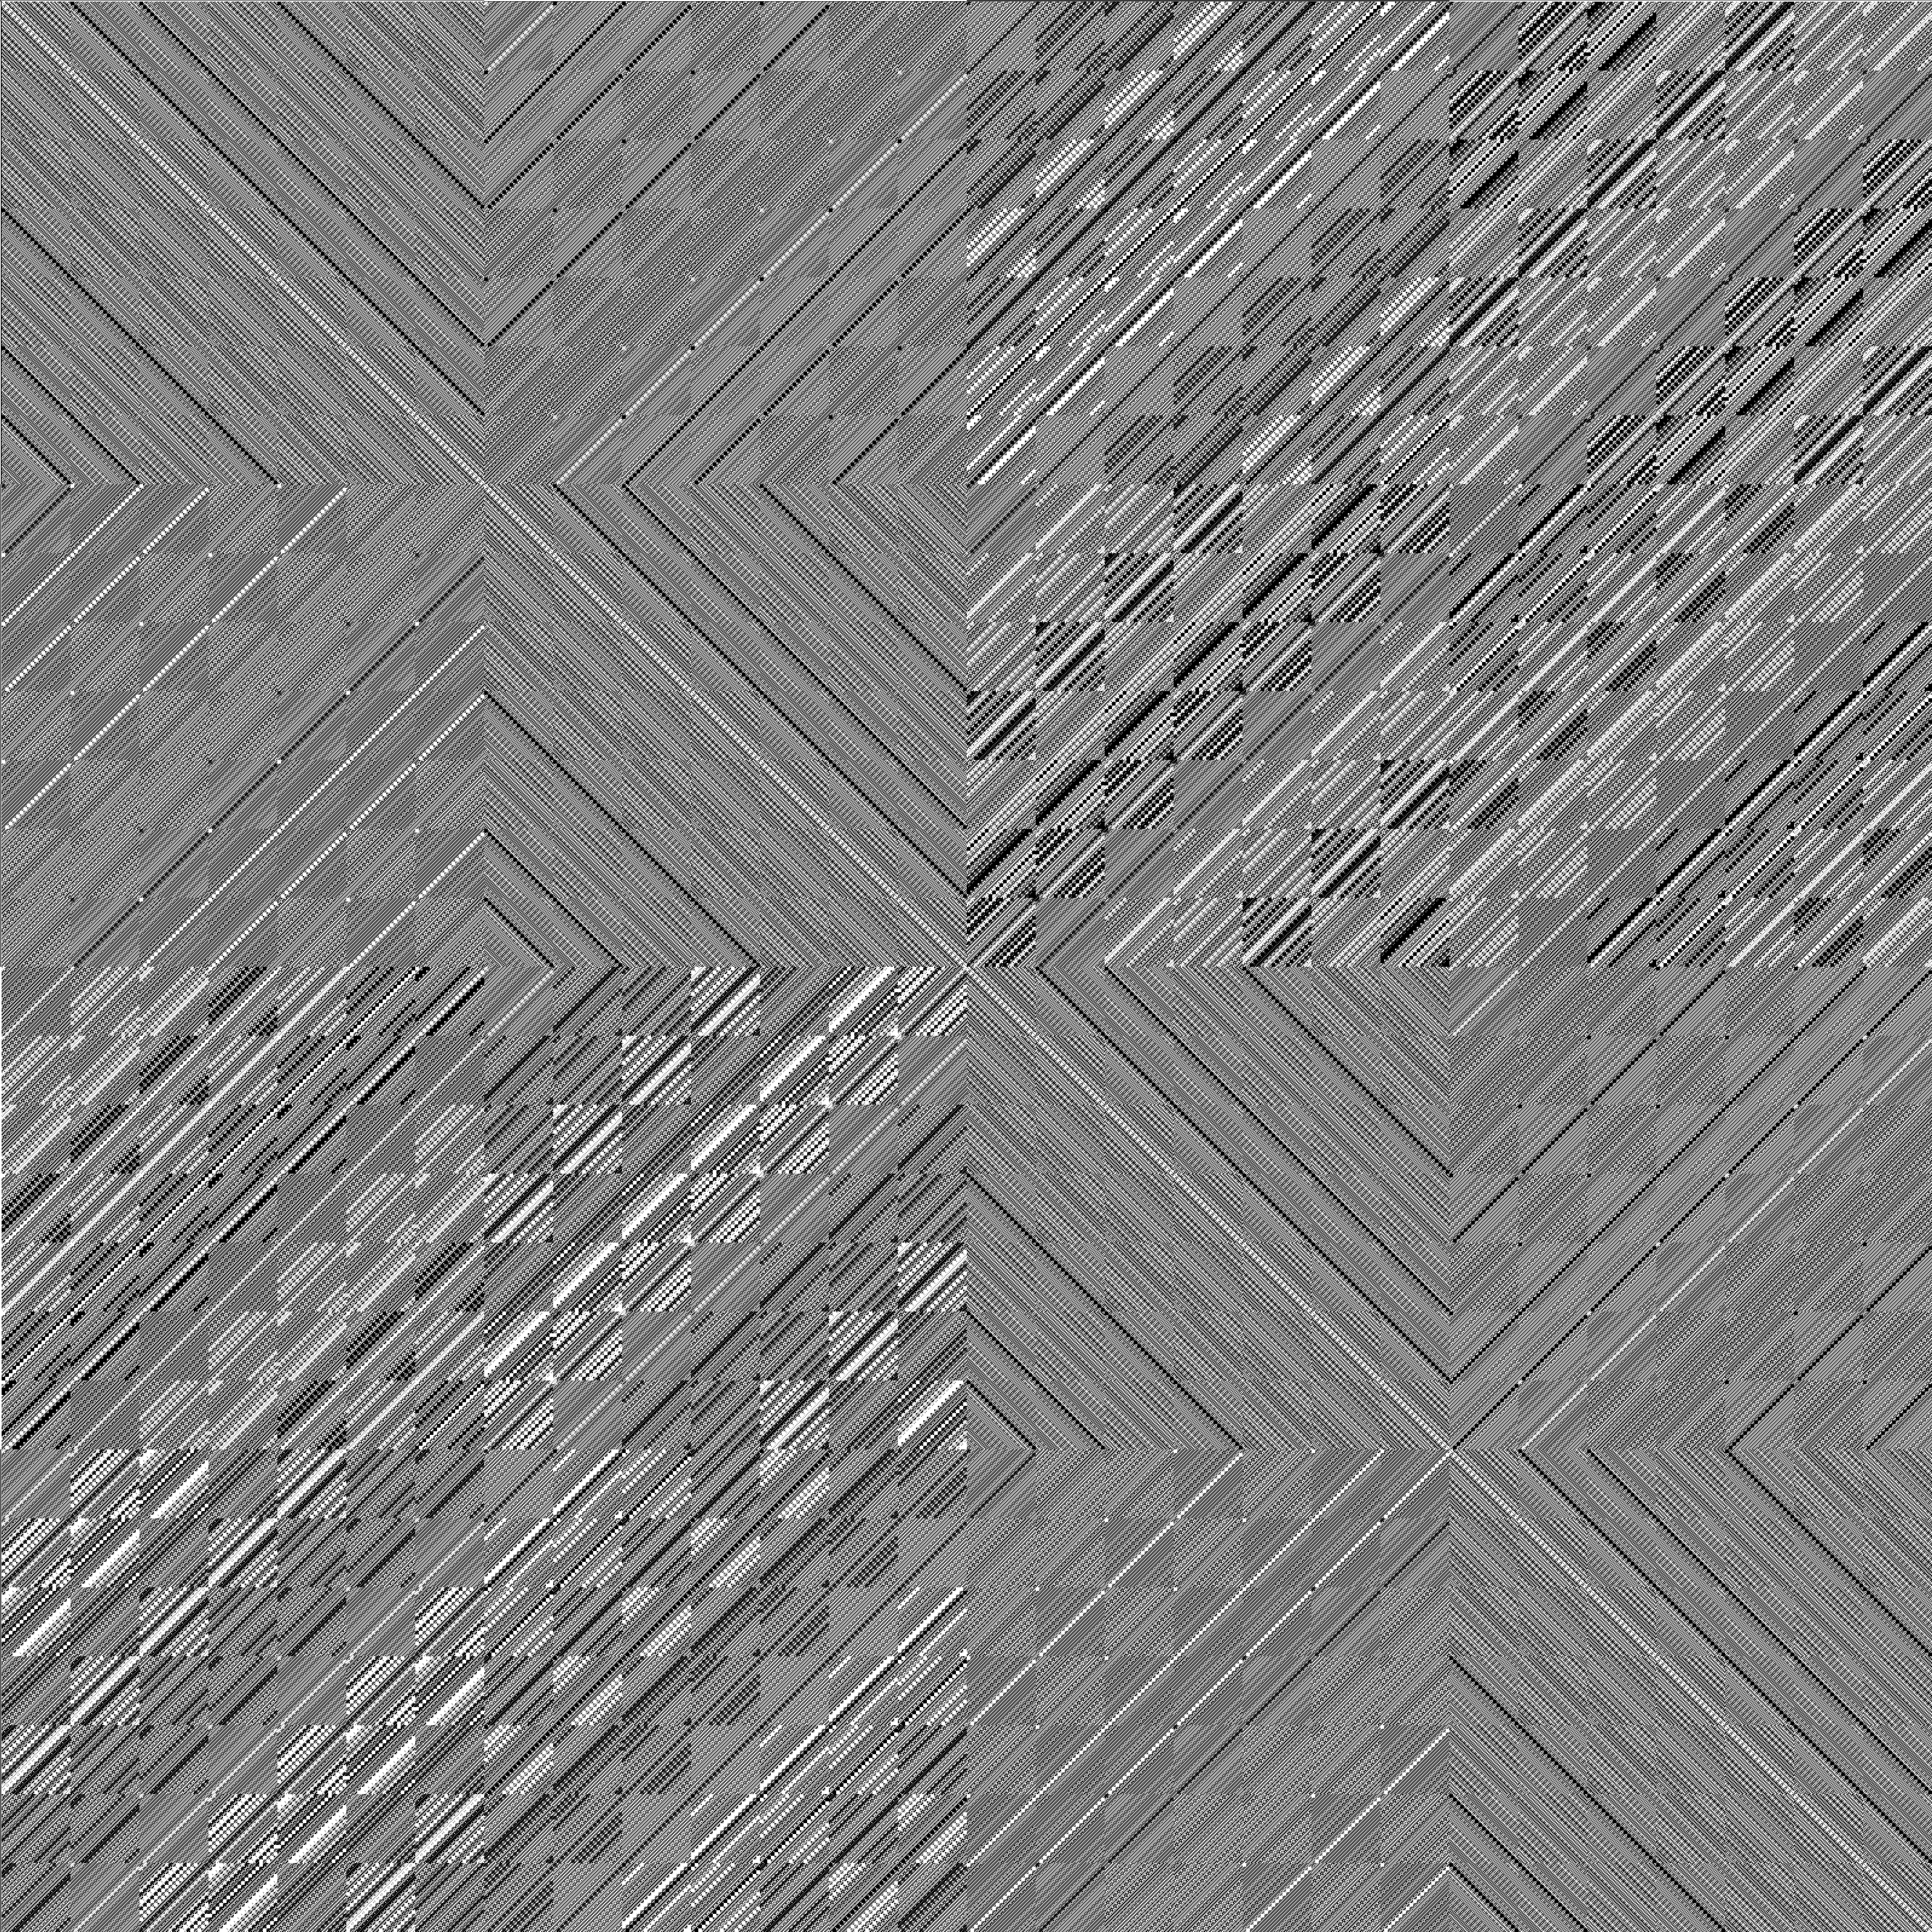
\includegraphics[width=\linewidth]{H4792.png}\\[2pt]
\small (a) The whole matrix
\end{minipage}\hfill
\begin{minipage}[b]{0.34\linewidth}\centering
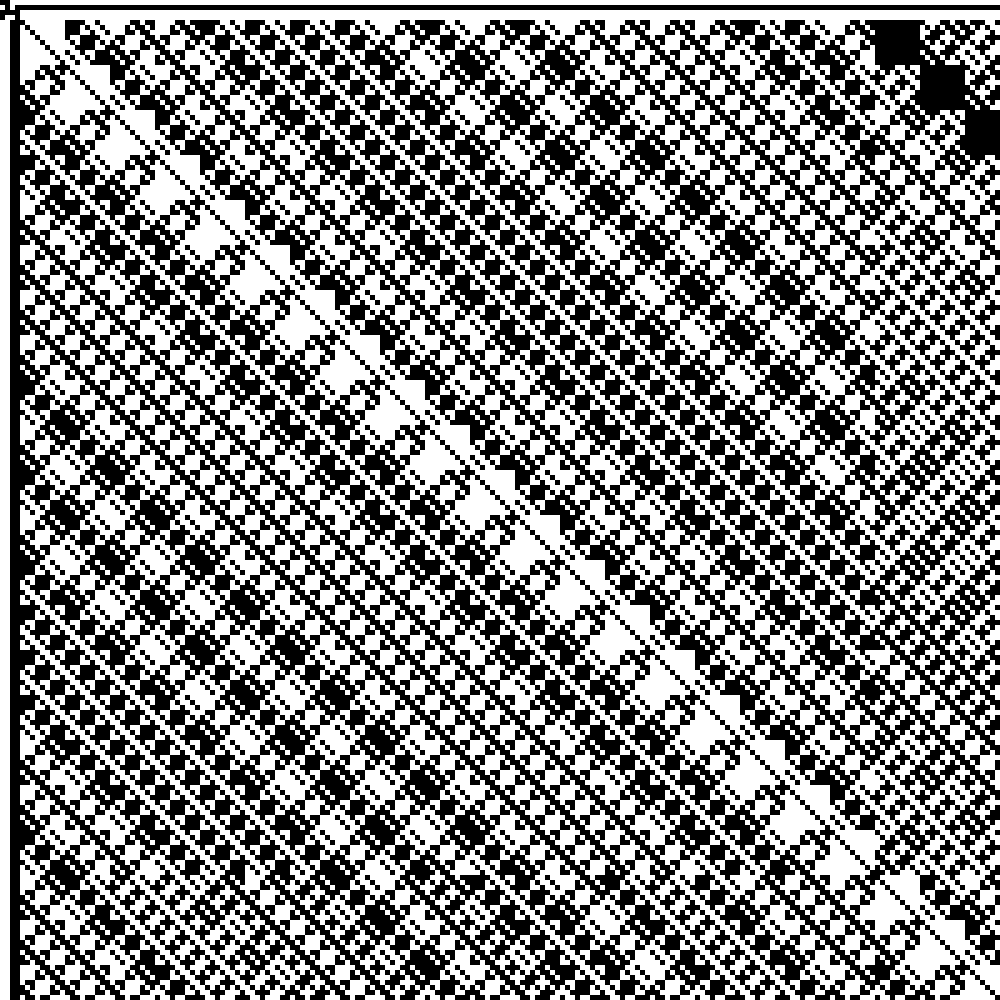
\includegraphics[width=\linewidth]{H4792-corner.png}\\[2pt]
\small (b) The top-left $200\times200$ corner
\end{minipage}
\caption{The Hadamard matrix $H$ of order $4792$, with $+1$ white and $-1$ black, in the row and column order of \Cref{thm:bordered}: the four border rows and columns come first, followed by the $4\times4$ array of blocks of size $1197$. The image is drawn from the published matrix (\Cref{sec:verification}) and agrees with it entry by entry.}
\label{fig:matrix}
\end{figure}

\paragraph{The construction.}
Let $G$ be a finite abelian group of odd order $m$. Suppose that four functions $a,b,c,d\colon G\to\{\pm1\}$ have periodic autocorrelations summing to $-4$ at every nonzero shift. Then a Goethals--Seidel array of the four group-developed matrices, with a border of width four, is a Hadamard matrix of order $4(m+1)$ (\Cref{thm:bordered}). Kumar calls this Spence's construction, and used it for his matrix of order $5912$ with $m=1477$ \cite{Kumar}. Bordered Goethals--Seidel arrays of this kind also appear in several of the constructions surveyed in \cite{EKLO}. Since the proof is short we give it in full. For order $4792$ we take $m=1197$ and
\[
G=\Z_7\times\Z_{19}\times\F_9 .
\]
\Cref{sec:functions} gives four functions on $G$ with the required autocorrelations. They are invariant under a group of multipliers of order $36$, which has $51$ orbits on $G$, so each function is described by $51$ signs. Kumar's search notes identify this group $G$ and this multiplier group as the most promising structure for $p=599$ \cite{Kumar}.

\paragraph{Verification.}
The proof of \Cref{thm:main} is \Cref{thm:bordered} together with a finite computation (\Cref{lem:paf}): for each of the $1196$ nonzero elements $t$ of $G$, count the ordered pairs in the four negative sets that differ by $t$. This takes a fraction of a second. We also checked the matrix itself. Three independent programs, one of them Kumar's, build or read all $4792^2$ entries and find $HH^{\T}=4792I$ exactly (\Cref{sec:verification}). The matrix, the certificate and the programs are available at \coderepo.

\paragraph{The search.}
\Cref{sec:search} describes how the functions were found. The search split the problem into $1141$ cases, discarded $617$ of them by exact tests on two quotients of $G$, and found the solution in one of the remaining cases. A second case gave a second solution. The correctness of \Cref{thm:main} does not depend on the search.

\paragraph{Notation.}
Groups are written additively. For a function $x\colon G\to\{\pm1\}$ we write $s_x=\sum_{g\in G}x(g)$ for its sign sum,
\[
P_x(t)=\sum_{g\in G}x(g)\,x(g+t)\qquad(t\in G)
\]
for its periodic autocorrelation, and $\dev x$ for the $G\times G$ matrix with entries $\dev x_{g,h}=x(h-g)$. We write $I$ and $J$ for the identity and all-ones matrices, $\one$ for the all-ones column vector, and $R$ for the $G\times G$ permutation matrix with $R_{g,h}=1$ exactly when $h=-g$. Matrices indexed by $G$ use a fixed ordering of $G$.

\section{The bordered array}\label{sec:array}

\begin{lemma}\label{lem:developed}
Let $G$ be a finite abelian group and let $x,y\colon G\to\{\pm1\}$. Then
\begin{enumerate}
\item\label{it:commute} $\dev x\dev y=\dev y\dev x$ and $\dev x^{\T}\dev y=\dev y\dev x^{\T}$;
\item\label{it:gram} $\dev x\dev x^{\T}=\dev x^{\T}\dev x$, and its $(g,h)$ entry is $P_x(g-h)$;
\item\label{it:reflect} $R^2=I$, $R^{\T}=R$, $R\dev xR=\dev x^{\T}$, and $\dev xR$ is symmetric;
\item\label{it:rowsum} $\dev x\one=\dev x^{\T}\one=s_x\one$.
\end{enumerate}
\end{lemma}

\begin{proof}
For a function $f\colon G\to\Z$ let $L_f$ be the matrix with entries $(L_f)_{g,h}=f(h-g)$. Then $(L_fL_{f'})_{g,h}=\sum_k f(k-g)f'(h-k)=\sum_u f(u)f'(h-g-u)$, which is symmetric in $f$ and $f'$ because $G$ is abelian, so all the matrices $L_f$ commute. Since $\dev x=L_x$ and $\dev x^{\T}=L_{\tilde x}$ with $\tilde x(g)=x(-g)$, this gives \ref{it:commute} and the first part of \ref{it:gram}. Next, $(\dev x\dev x^{\T})_{g,h}=\sum_k x(k-g)x(k-h)=\sum_u x(u)x(u+g-h)=P_x(g-h)$. For \ref{it:reflect}, $R$ is the matrix of the involution $g\mapsto-g$, and $(R\dev xR)_{g,h}=\dev x_{-g,-h}=x(g-h)=\dev x^{\T}_{g,h}$. Hence $(\dev xR)^{\T}=R\dev x^{\T}=R(R\dev xR)=\dev xR$. Finally every row and every column of $\dev x$ contains each value $x(u)$ exactly once.
\end{proof}

\begin{theorem}\label{thm:bordered}
Let $G$ be a finite abelian group of odd order $m$, and let $a,b,c,d\colon G\to\{\pm1\}$ satisfy
\begin{equation}\label{eq:paf}
P_a(t)+P_b(t)+P_c(t)+P_d(t)=-4\qquad\text{for every }t\in G\setminus\{0\}.
\end{equation}
Then $s_a,s_b,s_c,s_d\in\{\pm1\}$. Write $A,B,C,D$ for $\dev a,\dev b,\dev c,\dev d$ and $a,b,c,d$ also for the four sign sums, and put
\[
M=\begin{pmatrix}
A&BR&CR&DR\\
-BR&A&D^{\T}R&-C^{\T}R\\
-CR&-D^{\T}R&A&B^{\T}R\\
-DR&C^{\T}R&-B^{\T}R&A
\end{pmatrix},\qquad
S=\begin{pmatrix}
a&b&c&d\\
-b&a&d&-c\\
-c&-d&a&b\\
-d&c&-b&a
\end{pmatrix},
\]
\[
H=\begin{pmatrix}-S&S\otimes\one^{\T}\\ S\otimes\one&M\end{pmatrix}.
\]
Then $H$ is a Hadamard matrix of order $4(m+1)$.
\end{theorem}

The matrix $M$ is the Goethals--Seidel array \cite{GS} of the four group-developed matrices.

\begin{proof}
Each $P_x(0)$ equals $m$, so \eqref{eq:paf} gives $\sum_{t\in G}\bigl(P_a+P_b+P_c+P_d\bigr)(t)=4m-4(m-1)=4$. Since $\sum_tP_x(t)=s_x^2$, we get $s_a^2+s_b^2+s_c^2+s_d^2=4$. Each $s_x$ is odd because $m$ is odd, so each $s_x$ is $\pm1$. In particular every entry of $H$ is $\pm1$, and $H$ has order $4+4m$.

By \Cref{lem:developed}(\ref{it:gram}) and \eqref{eq:paf},
\begin{equation}\label{eq:sum}
AA^{\T}+BB^{\T}+CC^{\T}+DD^{\T}=4(m+1)I-4J.
\end{equation}

\emph{The array $M$.} We show $MM^{\T}=I_4\otimes\bigl(4(m+1)I-4J\bigr)$. By \Cref{lem:developed}(\ref{it:reflect}), $(XR)^{\T}=XR$ and $(X^{\T}R)^{\T}=RX=X^{\T}R$ for $X\in\{A,B,C,D\}$, and $XR\,YR=XY^{\T}$ for all such $X,Y$, as $RYR=Y^{\T}$; similarly $X^{\T}R\,Y^{\T}R=X^{\T}Y$ and $XR\,Y^{\T}R=XY$. A diagonal block of $MM^{\T}$ is the sum of the four terms $UU^{\T}$ over the blocks $U$ of one block row, and by these identities and \Cref{lem:developed}(\ref{it:gram}) each is one of $AA^{\T},BB^{\T},CC^{\T},DD^{\T}$, each appearing once. So every diagonal block equals \eqref{eq:sum}. For the off-diagonal blocks we compute the $(1,2)$ block; the other five are the same computation with the letters permuted:
\begin{align*}
&A(-BR)^{\T}+BR\,A^{\T}+CR\,(D^{\T}R)^{\T}+DR\,(-C^{\T}R)^{\T}\\
&\qquad=-ABR+BRA^{\T}+CR\,D^{\T}R-DR\,C^{\T}R .
\end{align*}
Here $BRA^{\T}=B(RA^{\T}R)R=BAR$, $CR\,D^{\T}R=CD$ and $DR\,C^{\T}R=DC$, so the block is $(BA-AB)R+CD-DC=0$ by \Cref{lem:developed}(\ref{it:commute}).

\emph{The border.} The matrix $S$ satisfies $SS^{\T}=(a^2+b^2+c^2+d^2)I_4=4I_4$, by a direct check of its rows. Let $E=I_4\otimes\one$, the $4m\times4$ matrix whose $j$th column is the indicator of the $j$th block of columns. By \Cref{lem:developed}(\ref{it:rowsum}), every block of $M$ has constant row sums, equal to the corresponding entry of $S$; for example $D^{\T}R\one=D^{\T}\one=d\one$. Hence $ME=ES$, that is, $M(I_4\otimes\one)=S\otimes\one$.

\emph{The Gram matrix of $H$.} Write $H=\begin{pmatrix}H_{11}&H_{12}\\H_{21}&H_{22}\end{pmatrix}$ as displayed. Then
\begin{align*}
H_{11}H_{11}^{\T}+H_{12}H_{12}^{\T}&=SS^{\T}+(SS^{\T})\otimes(\one^{\T}\one)=4(m+1)I_4,\\
H_{11}H_{21}^{\T}+H_{12}H_{22}^{\T}&=-(SS^{\T})\otimes\one^{\T}+(ME\,S^{\T})^{\T}=-4E^{\T}+4E^{\T}=0,\\
H_{21}H_{21}^{\T}+H_{22}H_{22}^{\T}&=(SS^{\T})\otimes J+MM^{\T}=4(m+1)I_{4m}.
\end{align*}
In the second line we used $H_{12}H_{22}^{\T}=(S\otimes\one^{\T})M^{\T}=(M(S^{\T}\otimes\one))^{\T}$, $S^{\T}\otimes\one=ES^{\T}$ and $ME\,S^{\T}=ESS^{\T}=4E$. In the third line, $(SS^{\T})\otimes J=4\,I_4\otimes J$ and $MM^{\T}=I_4\otimes\bigl(4(m+1)I-4J\bigr)$. So $HH^{\T}=4(m+1)I$.
\end{proof}

The condition \eqref{eq:paf} has two standard reformulations. Let $D_x=\{g:x(g)=-1\}$ be the negative set of $x$ and $\lambda_x(t)=|\{(g,h)\in D_x^2:h-g=t\}|$. Since $x=1-2\cdot1_{D_x}$,
\begin{equation}\label{eq:differences}
P_x(t)=m-4|D_x|+4\lambda_x(t).
\end{equation}
So \eqref{eq:paf} says that the four negative sets form supplementary difference sets: every nonzero $t$ arises the same number $\lambda=|D_a|+|D_b|+|D_c|+|D_d|-m-1$ of times as a difference of two elements of one of the sets. Equivalently, by Fourier analysis on $G$, $|\hat a(\chi)|^2+|\hat b(\chi)|^2+|\hat c(\chi)|^2+|\hat d(\chi)|^2=4(m+1)$ for every nontrivial character $\chi$ of $G$, where $\hat x(\chi)=\sum_gx(g)\chi(g)$. The search in \Cref{sec:search} uses the second form on quotients of $G$.

\section{The four functions}\label{sec:functions}

Let $K=\Z_7\times\Z_{19}$ and let $\F_9=\F_3[i]$ with $i^2=-1$. We identify $\F_9$ with $\F_3^2$ by $u+vi\mapsto(u,v)$, and write the elements of
\[
G=K\times\F_9=\Z_7\times\Z_{19}\times\F_3^2
\]
as $(x,y,u,v)$ with $x\in\Z_7$, $y\in\Z_{19}$ and $u,v\in\F_3=\{0,1,2\}$. The group has order $m=7\cdot19\cdot9=1197$, and $4(m+1)=4792$.

\paragraph{Multipliers.}
The map $\mu(x,y)=(2x,4y)$ is an automorphism of $K$ of order $9$: the element $2$ has order $3$ in $\Z_7^\times$ and $4$ has order $9$ in $\Z_{19}^\times$. Multiplication by $i$, which is $(u,v)\mapsto(-v,u)$, is an automorphism of $\F_9$ of order $4$. The group $\langle\mu\rangle\times\langle i\rangle$ of order $36$ acts on $G$ coordinatewise. Its orbits on $K$ are $\{(0,0)\}$, two orbits of size $3$ in $\Z_7^\times\times\{0\}$, two orbits of size $9$ in $\{0\}\times\Z_{19}^\times$, and $12$ orbits of size $9$ in $\Z_7^\times\times\Z_{19}^\times$: $17$ orbits in all. Order them by their least element in the lexicographic order. Their least elements are
\[
\begin{array}{c@{\quad}ccccccccc}
j&0&1&2&3&4&5&6&7&8\\
(x,y)&(0,0)&(0,1)&(0,2)&(1,0)&(1,1)&(1,2)&(1,4)&(1,5)&(1,8)\\[3pt]
j&9&10&11&12&13&14&15&16\\
(x,y)&(1,10)&(3,0)&(3,1)&(3,2)&(3,4)&(3,5)&(3,8)&(3,10)
\end{array}
\]
and we write $O_j$ for the orbit with index $j$. The orbits of $\langle i\rangle$ on $\F_9$ are $F_0=\{0\}$, the set $F_1=\{\pm1,\pm i\}$ of nonzero squares, which are the points with exactly one nonzero coordinate, and the set $F_2=\{\pm1\pm i\}$ of nonsquares, which are the points with two nonzero coordinates. So the $51$ orbits of the multiplier group on $G$ are the products $O_j\times F_k$.

\paragraph{The functions.}
Each of the four functions $a,b,c,d$ is constant on these $51$ orbits. For $x\in\{a,b,c,d\}$ and $k\in\{0,1,2\}$ let $w_{x,k}$ be the integer in \Cref{tab:masks}. The value of $x$ on $O_j\times F_k$ is $-1$ if bit $j$ of $w_{x,k}$ is set, counting from the least significant bit as bit $0$, and $+1$ otherwise.

\begin{table}[ht]
\centering
\begin{tabular}{@{}ccccrr@{}}
\toprule
Function & $F_0$ (origin) & $F_1$ (squares) & $F_2$ (nonsquares) & $|D_x|$ & $s_x$ \\
\midrule
$a$ & \texttt{0c85b} & \texttt{1c32a} & \texttt{03cdc} & $598$ & $1$ \\
$b$ & \texttt{08573} & \texttt{07c3c} & \texttt{187c2} & $598$ & $1$ \\
$c$ & \texttt{08328} & \texttt{09e3d} & \texttt{16d4b} & $599$ & $-1$ \\
$d$ & \texttt{04ad2} & \texttt{03e65} & \texttt{1991b} & $599$ & $-1$ \\
\bottomrule
\end{tabular}
\caption{The twelve masks $w_{x,k}$, in hexadecimal, with the size of each negative set and each sign sum. Bit $j$ of $w_{x,k}$ gives the sign of $x$ on $O_j\times F_k$.}
\label{tab:masks}
\end{table}

For example, the mask $w_{a,0}=\texttt{0c85b}$ has bits $0,1,3,4,6,11,14$ and $15$ set. So $a(x,y,0,0)=-1$ exactly when $(x,y)$ lies in one of $O_0,O_1,O_3,O_4,O_6,O_{11},O_{14},O_{15}$.

\begin{lemma}\label{lem:paf}
The functions $a,b,c,d$ of \Cref{tab:masks} satisfy \eqref{eq:paf} on $G$: with the notation of \eqref{eq:differences}, $\lambda_a(t)+\lambda_b(t)+\lambda_c(t)+\lambda_d(t)=1196$ for every nonzero $t\in G$.
\end{lemma}

\begin{proof}
This is a finite computation. The four negative sets have sizes $598,598,599,599$, in total $2394$. A program expands the masks, enumerates all $598^2+598^2+599^2+599^2=1\,432\,810$ ordered pairs $(g,h)$ in the four negative sets, and tallies $h-g$. It finds $2394$ pairs with $h-g=0$ and exactly $1196$ for each of the $1196$ nonzero elements. By \eqref{eq:differences}, $\sum_xP_x(t)=4\cdot1197-4\cdot2394+4\cdot1196=-4$ for $t\ne0$.
\end{proof}

The multiplier symmetry reduces the check. If $\sigma$ is an automorphism of $G$ and $x\circ\sigma=x$, then $P_x(\sigma t)=\sum_gx(\sigma g)x(\sigma g+\sigma t)=P_x(t)$. So the sum in \eqref{eq:paf} is constant on the $50$ nonzero orbits $O_j\times F_k$, and it suffices to check one shift in each. The programs check all $1196$ shifts.

\begin{proof}[Proof of \Cref{thm:main}]
Apply \Cref{thm:bordered} to the group $G$ of order $1197$ and the functions of \Cref{tab:masks}, which satisfy \eqref{eq:paf} by \Cref{lem:paf}. The result is a Hadamard matrix of order $4\cdot1198=4792$.
\end{proof}

\section{Verification}\label{sec:verification}

The four sign strings, the full matrix $H$ and the programs used below are available at \coderepo. The matrix is stored as text, one row of $H$ per line, with the entries $1$ and $-1$ separated by commas and each line ending with a line feed. The rows and columns are in the order of \Cref{thm:bordered}: the four border rows, then the $4\cdot1197$ rows of $(S\otimes\one\ \ M)$, with $G$ in lexicographic order of $(x,y,u,v)$. This text has SHA-256 hash
\begin{center}\footnotesize
\texttt{5953fc1f8ad4cfcd38c782b9e7be909af4b0d7dc5bd94073a98dc4765e57eab6}.
\end{center}
We ran four checks. The first proves \Cref{lem:paf}. The other three check the matrix directly, so they do not rely on \Cref{thm:bordered}.
\begin{enumerate}
\item \emph{Differences.} A program that uses only the Python standard library checks that the twelve masks expand to the four sign strings, and counts the differences as in the proof of \Cref{lem:paf}.
\item \emph{Row pairs.} A second program builds every entry of $H$ from an explicit formula, packs each row into an integer, and checks all $\binom{4792}{2}=11\,479\,236$ pairs of distinct rows by exclusive-or and population count. Every pair of rows differs in exactly $2396$ positions, so every two distinct rows are orthogonal. It also writes the matrix it builds in the text form above, and the SHA-256 hash agrees.
\item \emph{The array.} A third, separately written program builds $A,B,C,D$, $M$, $S$ and $H$ from the masks by the matrix formulas of \Cref{thm:bordered} and computes $HH^{\T}$. It also reads the stored matrix and computes its Gram matrix. Both Gram matrices equal $4792I$, and the matrix built from the masks equals the stored matrix entry by entry. The products are computed in double precision; every partial sum is an integer of absolute value at most $4792$, so the arithmetic is exact.
\item \emph{Kumar's checker.} Kumar's standalone verifier \cite{Kumar}, written in C, reads the stored matrix, checks that every entry is $\pm1$, and computes all $11\,484\,028$ inner products of pairs of rows, the diagonal included. It reports no violations. As a control, changing a single entry makes it report $4791$ violations.
\end{enumerate}
Each check takes a few seconds.

\section{How the functions were found}\label{sec:search}

This section records the search. It is not needed for the proof.

For orders $8p$, Kumar \cite{Kumar} studied Spence-type structures over groups of odd order $2p-1$, with the four functions constant on the orbits of a group of multipliers, and estimated their cost. For $p=599$ his best remaining structure was the group $G=\Z_7\times\Z_{19}\times\F_9$ with a multiplier group of order $36$, at an estimated $1.5\cdot10^3$ core-hours. The same approach gave his matrix of order $5912$ over $\Z_{211}\times\F_7$. Before searching at order $4792$ we reran his order-$5912$ search from the recorded seed and recovered his matrix.

A function invariant under the multipliers is determined by its three values on each fibre $\{k\}\times\F_9$, at $0$, on the squares and on the nonsquares. Following Kumar, the search first fixed some coarse numerical data of each of the four functions, such as sums of its values over parts of the fibres. Up to the symmetries of the problem there are $1141$ possibilities for these data, which we call cases. Projecting \eqref{eq:paf} to the quotients $\Z_7\times\F_9$ and $\Z_{19}\times\F_9$ of $G$, in the Fourier form at the end of \Cref{sec:array}, gives exact necessary conditions, and $524$ of the $1141$ cases satisfy them. For a surviving case the search enumerated candidate functions block by block, matched the four blocks on their projected autocorrelations, and tested each match against \eqref{eq:paf} on all of $G$.

The search ran on local CPUs with two choices of multiplier on $K$, $(2,4)$ and $(2,5)$, which give the same projected conditions. In all, $250$ cases for $(2,4)$ and $80$ for $(2,5)$ ended without a solution, and two cases for $(2,4)$ gave solutions. Case $268$ gave the functions of \Cref{tab:masks}. A clean rebuild and rerun of that case gave the same four sign strings. Case $523$ for $(2,4)$ gave a second solution, whose negative sets all have size $599$. It also passes the first two checks of \Cref{sec:verification}. We have not tested whether the two Hadamard matrices are equivalent under signed permutations of rows and columns. The second certificate and the search programs are also available at \coderepo.

\section{Remarks}\label{sec:remarks}

Order $2396=4\cdot599$, the smallest open order, is still open. Kumar \cite{Kumar} discusses which structures remain for it. Of the orders $8p$ below $10\,000$ in Kumar's list, only $5752=8\cdot719$ is now open. For $p=719$ the corresponding group has order $1437$, and Kumar reports that several structures of this type are already excluded there.

\section*{Acknowledgements}
This work builds directly on Kishan Kumar's public search programs, search records and verifier \cite{Kumar}, and the structure used here was identified in his search records. We are grateful to him for making them public.

\begin{thebibliography}{99}\small
\bibitem{EKLO} R.~Egan, I.~Kotsireas, S.~London and P.~\'O~Cath\'ain, \emph{Recent progress in the construction of Hadamard matrices}, arXiv:2610.27175v2 (2026).
\bibitem{Explorer} Hadamard Matrix Explorer, \emph{Unknown orders}, \url{https://www.math74.com/Hadamard/unknown.html}, accessed 25 November 2026.
\bibitem{GS} J.-M.~Goethals and J.\,J.~Seidel, \emph{A skew Hadamard matrix of order 36}, J.\ Austral.\ Math.\ Soc.\ \textbf{11} (1970), 343--344.
\bibitem{Hadamard} J.~Hadamard, \emph{R\'esolution d'une question relative aux d\'eterminants}, Bull.\ Sci.\ Math.\ (2) \textbf{17} (1893), 240--246.
\bibitem{KTR} H.~Kharaghani and B.~Tayfeh-Rezaie, \emph{A Hadamard matrix of order 428}, J.\ Combin.\ Des.\ \textbf{13} (2005), 435--440.
\bibitem{Kumar} K.~Kumar, \emph{New Hadamard matrices}, search programs, records and verifier, \url{https://github.com/vatskishan03/Hadamard}, 2026, accessed 25 November 2026.
\bibitem{Paley} R.\,E.\,A.\,C.~Paley, \emph{On orthogonal matrices}, J.\ Math.\ Phys.\ \textbf{12} (1933), 311--320.
\bibitem{SY} J.~Seberry and M.~Yamada, \emph{Hadamard matrices, sequences, and block designs}, in: J.\,H.~Dinitz and D.\,R.~Stinson (eds.), Contemporary Design Theory: A Collection of Surveys, Wiley, New York, 1992, 431--560.
\bibitem{Sylvester} J.\,J.~Sylvester, \emph{Thoughts on inverse orthogonal matrices, simultaneous sign successions, and tessellated pavements in two or more colours, with applications to Newton's rule, ornamental tile-work, and the theory of numbers}, Philos.\ Mag.\ (4) \textbf{34} (1867), 461--475.
\end{thebibliography}

\end{document}
